\documentclass[9pt]{beamer}
\usecolortheme{beaver}
\setbeamertemplate{navigation symbols}{}
\setbeamercolor{block title}{bg=white!95!black,fg=black}
\defbeamertemplate{description item}{align left}{\insertdescriptionitem\hfill}
    \setbeamertemplate{description item}[align left]
\usepackage{tikz}

\usepackage[outputdir=../build]{minted}
\usepackage{tcolorbox}
\tcbuselibrary{minted,skins}

% Patch to fix https://github.com/T-F-S/tcolorbox/issues/12
\makeatletter
\def\tcb@minted@input@listing#1#2#3#4{%
  \edef\temp@a{#4}%
  \ifx\temp@a\@empty%
  \else%
    \toks@=\expandafter{#4}%
    \edef\tcb@temp{\noexpand\usemintedstyle{\the\toks@}}%
    \tcb@temp%
  \fi%
  \toks@=\expandafter{#1}%
  \edef\tcb@temp{\noexpand\inputminted[\the\toks@]}%
  \IfFileExists{\minted@outputdir#3}%
    {\tcb@temp{#2}{\minted@outputdir#3}}%
    {\tcb@temp{#2}{#3}}%
}
\makeatother

\newtcblisting{ccode}[2][]{%
  listing engine=minted,
  minted language=#2,
  minted options={breaklines,breakanywhere,fontsize=\scriptsize,gobble=8},
  listing only,
  before skip=0pt,
  after skip=8pt,
  left skip=0pt,
  right skip=0pt,
  size=fbox,
  sharp corners,
  %colframe=white!75!black,
  colframe=white,
  boxrule=0pt,
  frame hidden,
  #1
}


\newtcbinputlisting[]{\inputcode}[3][]{%
  listing engine=minted,
  minted language=#2,
  minted options={breaklines,breakanywhere,fontsize=\scriptsize,#1},
  listing file={#3},
  listing only,
  size=fbox,
  before skip=0pt,
  after skip=10pt,
  left skip=0pt,
  right skip=0pt,
  sharp corners,
  %colframe=white!75!black,
  colframe=white,
  boxrule=0pt,
  frame hidden
}


\title{Small Sparse Matrix Multiplications\\ on Knights Landing}
\author{Nathan Brei}
\institute{Technical University of Munich}
\date\today

\begin{document}
\begin{frame}
  \titlepage
\end{frame}



\begin{frame}
  \frametitle{Motivation}
  
  \begin{block}{SeisSol}
    Simulates earthquakes, specifically, dynamic rupture processes and seismic wave propagation over an unstructured tetrahedral mesh. 
  \end{block}

  \begin{block}{ADER-DG}
    A numerical method which uses Discontinuous Galerkin discretization in space and ADER discretization in time. It avoids a global system matrix, using local element matrix operations instead.
  \end{block}

  \begin{block}{Small Sparse Matrix Multiplications}
    The compute kernels resemble the operation shown below, applied recursively. Different sparsity patterns are used, but they are all known at compile time.
  \end{block}

  \centering
  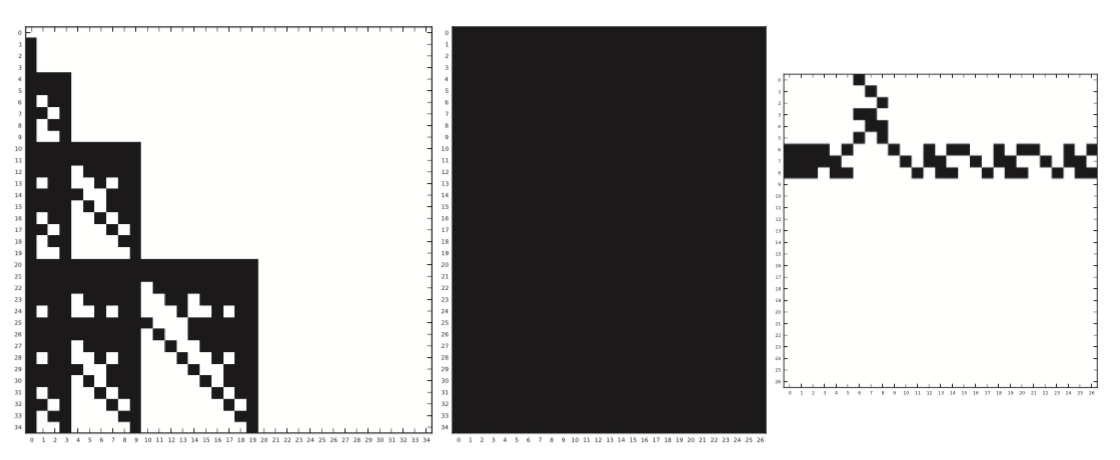
\includegraphics[height=3cm]{images/seissol_visc.png}

\end{frame}

\begin{frame}
  \frametitle{SeisSol Compute Kernels}
  \begin{block}{Element update}
  \centering
  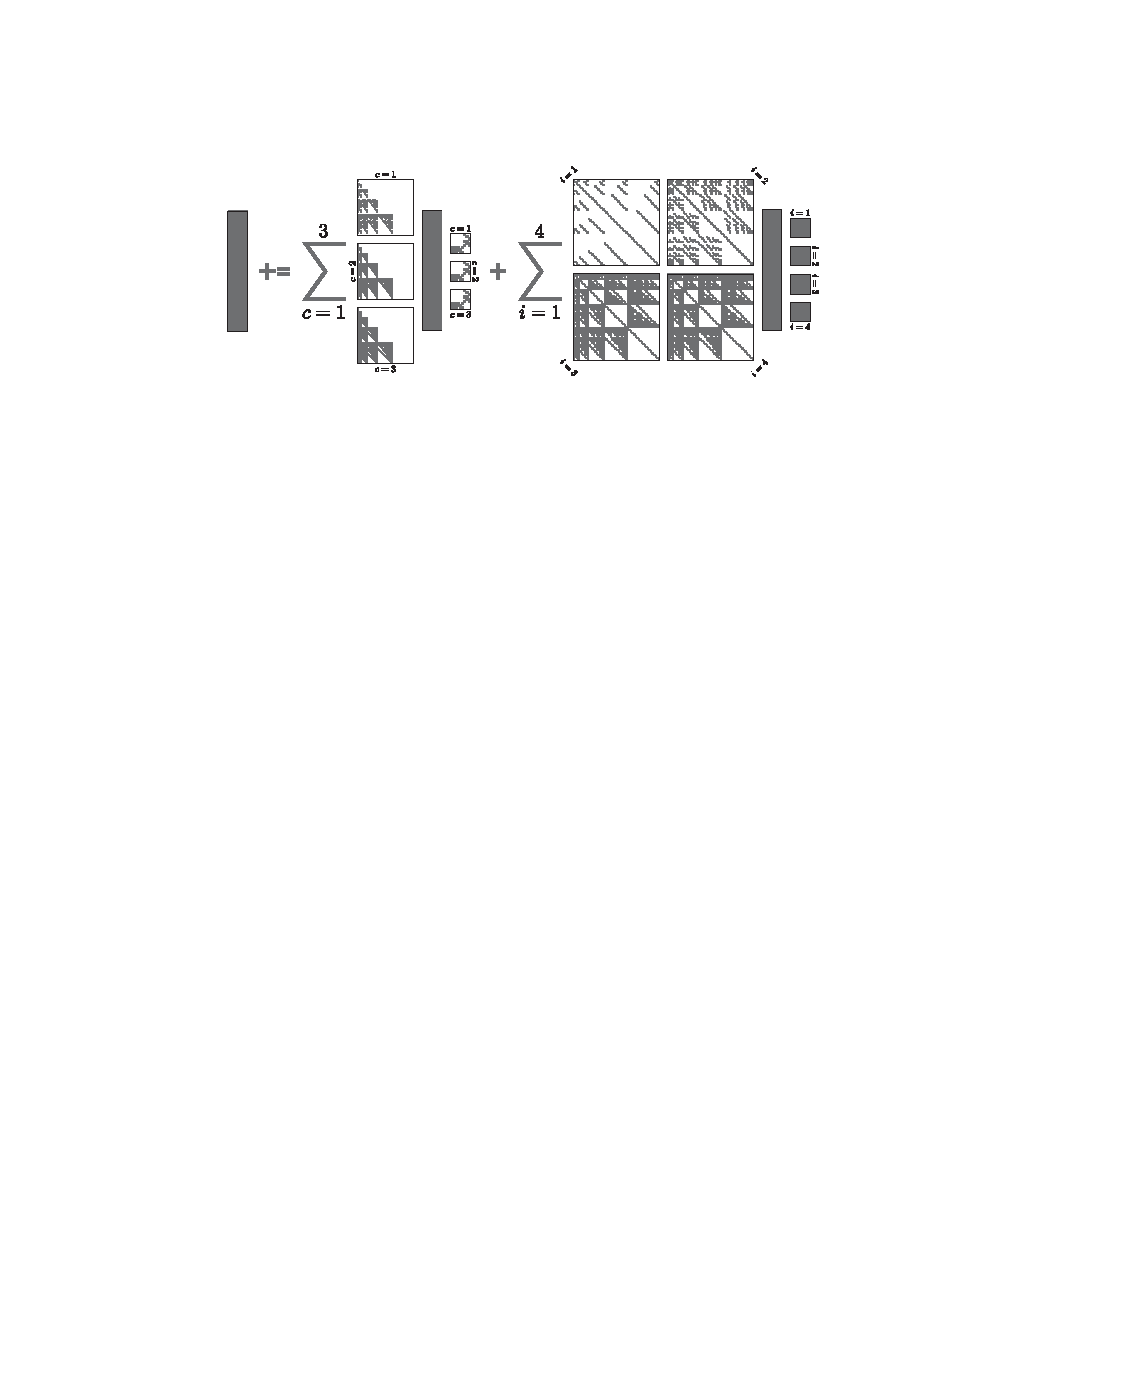
\includegraphics[height=3cm]{images/seissol_elem.pdf}
  \end{block}
  \begin{block}{Time integration}
  \centering
  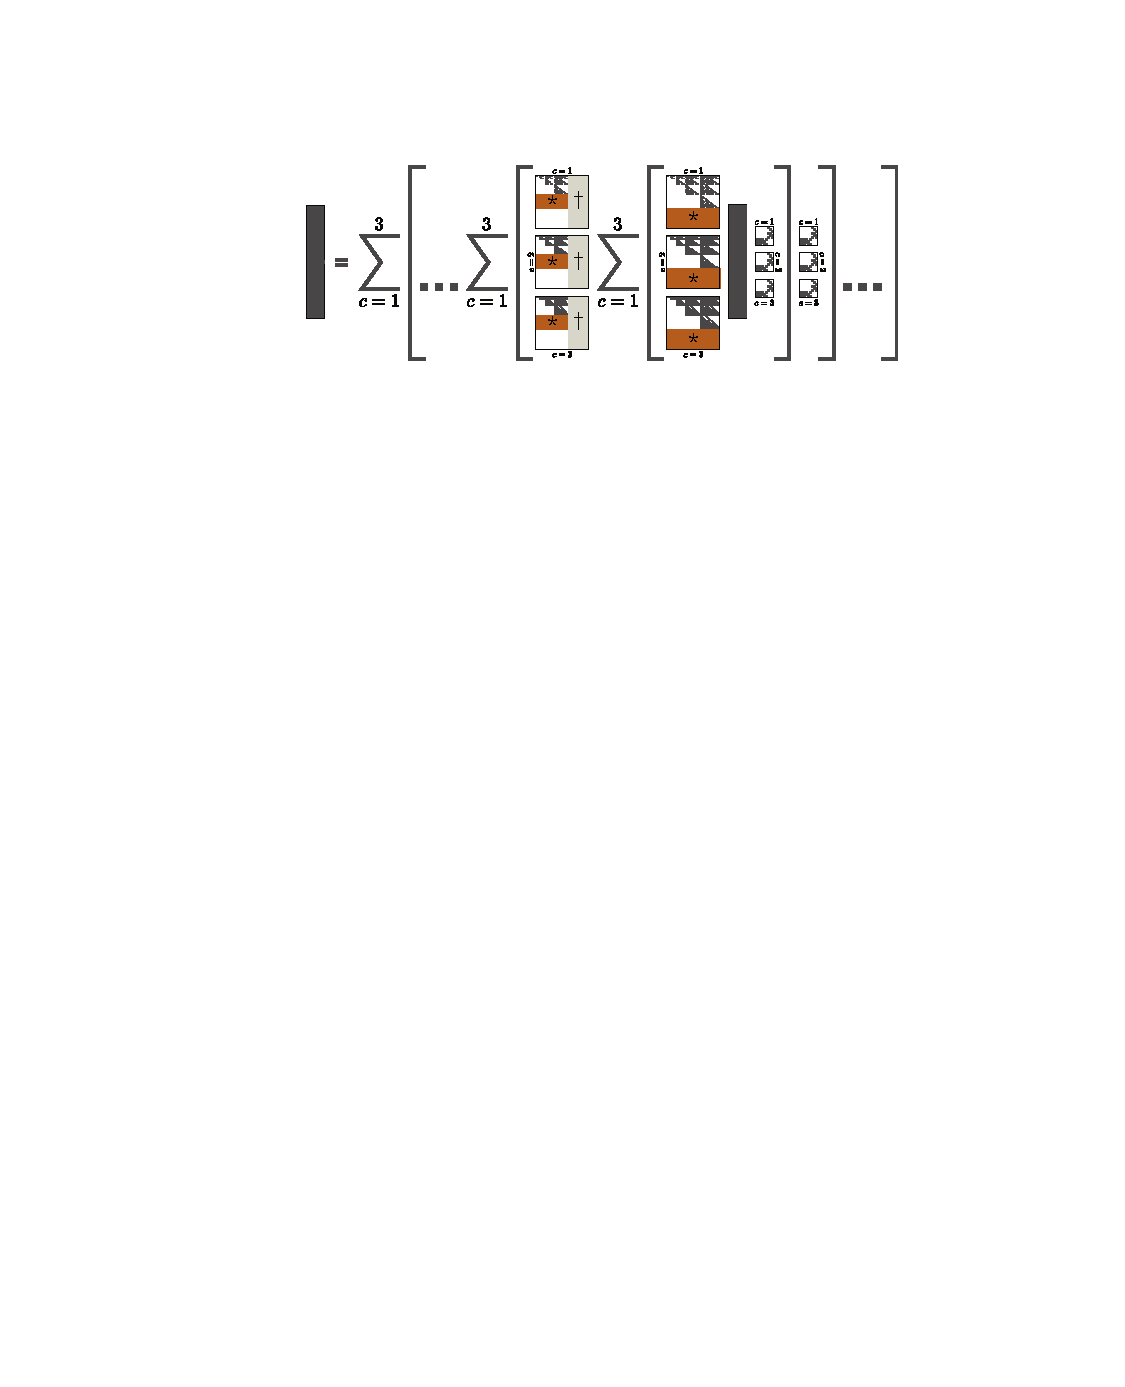
\includegraphics[height=3cm]{images/seissol_ader.pdf}
  \end{block}
  %\begin{block}{Neighbor updates}
  %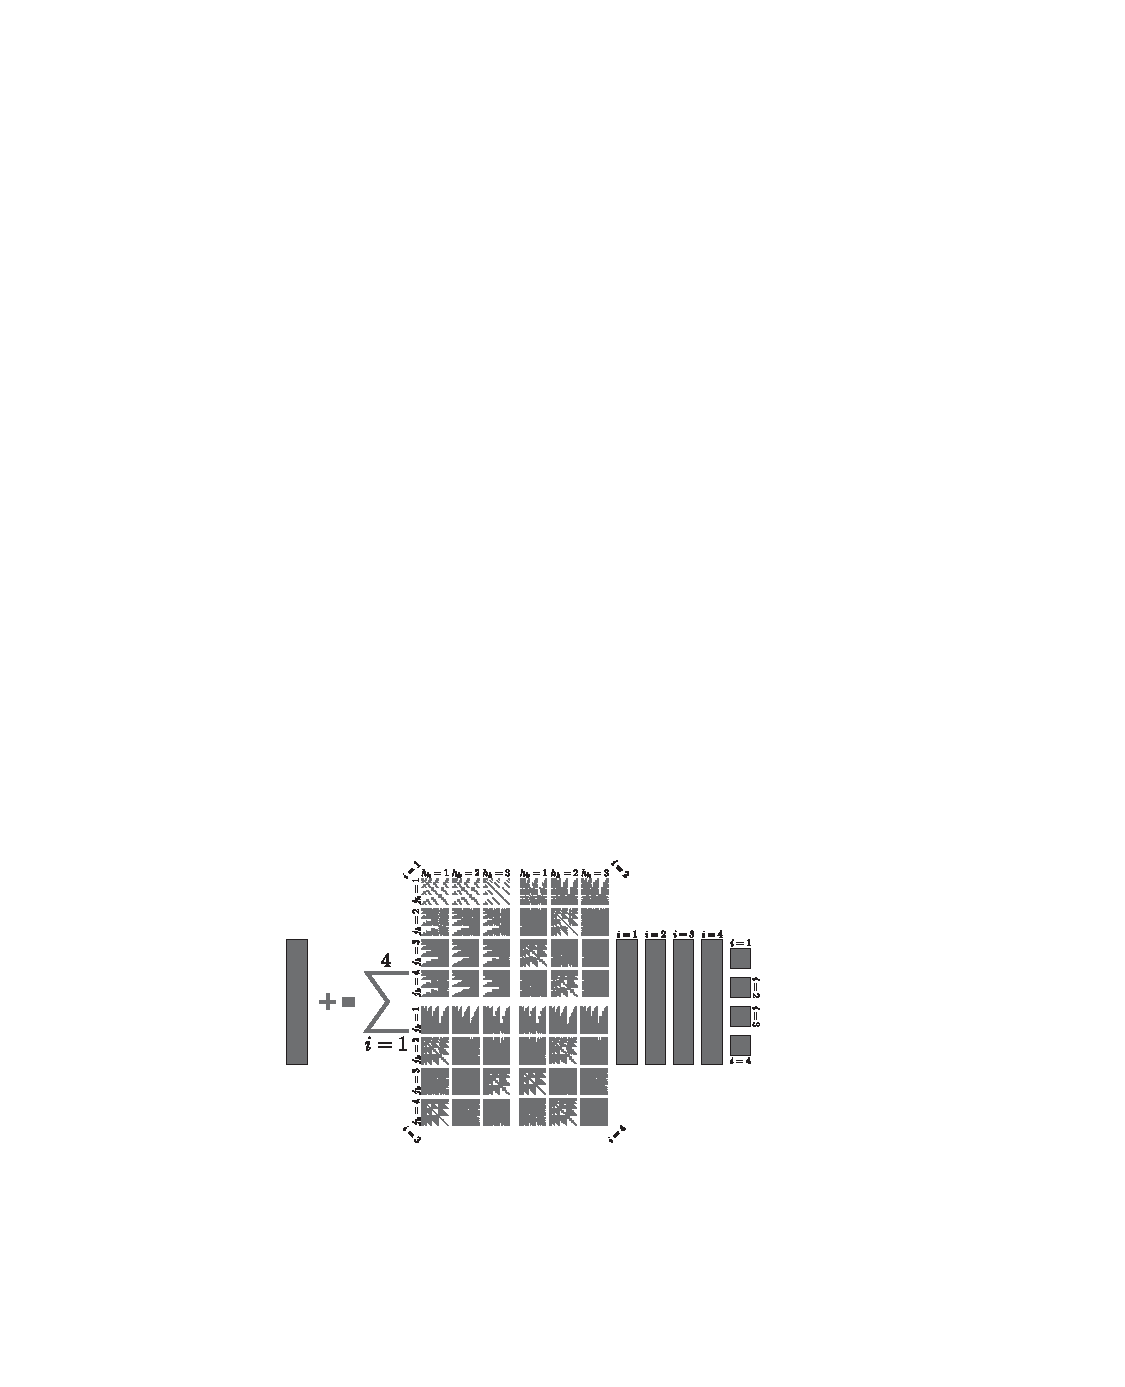
\includegraphics[height=3cm]{images/seissol_flux.pdf}
  %\end{block}

\end{frame}


\begin{frame}
  \frametitle{Knights Landing}
  \begin{block}{KNL is the 2nd-generation Intel Xeon Phi many-core processor}
    \begin{itemize}
    \item A standalone processor (not just a coprocessor or GPU) which supports the entire x86 instruction set along with AVX512 extensions.
    \item Organized into a 2D grid of up to 36 tiles, each containing 2 cores and a 1MB shared L2 cache
    \item 4 threads/core $\implies$ up to 288 threads/processor
    \item 32 vector registers holding 8 doubles/register
    \item Fused-multiply-add instruction $(=:FMA)$ with mask registers and implicit broadcast
    \item 2 vpus/core, 16 double ops/vpu/cycle, 1.3e9 cycles/sec \\ $\implies$ 3 double TFlop peak performance

    \end{itemize}
  \end{block}
  \begin{block}{KNL greatly prefers large dense matrix operations to small sparse ones}
    \begin{itemize}
    \item Scalar operations limited to 1/8 peak performance
    \item Bottleneck with vector stores: 64B/cycle
    \item Bottleneck with instruction cache, decoder: min(16B/cycle, 2 instructions)
    \item \textbf{Out-of-order execution pipeline can only issue 2 instructions per cycle}
    \end{itemize}
  \end{block}
\end{frame}

\begin{frame}
  \frametitle{Past approaches used in SeisSol}
  \begin{block}{Standard compressed-sparse-column multiplication}
    \begin{itemize}
      \item[$+$] General and widely applicable.
      \item[$+$] Algorithm uses a (small) constant number of instructions.
      \item[$-$] Requires performing index lookups: More memory movement, loops, logic.
      \item[$-$] Disregards the fact that the sparsity pattern is known at compile time.
    \end{itemize}
  \end{block}

  \begin{block}{Sparsity pattern unrolled into instruction stream}
    \begin{itemize}
    \item[$+$] Index lookups removed completely
    \item[$+$] $dense \times sparse$ case can be vectorized perfectly 
    \item[$-$] Generates one FMA instruction for every nonzero
    \item[$-$] (Implementation) Memory access pattern is suboptimal on KNL
    \item[$-$] (Implementation) Compiler struggles to generate efficient assembly
    \end{itemize}
  \end{block}
\end{frame}

\begin{frame}
  \frametitle{Present and future approaches}
  \begin{block}{Dense matrix multiplication}
    \begin{itemize}
    \item[$+$] Memory access patterns and register blockings optimized for KNL
    \item[$+$] (Implementation) Code generator emits assembly directly 
    \item[$-$] Filling in zero entries wastes both flops and memory bandwidth
    \end{itemize}
  \end{block}

  \begin{block}{My approach}
    \begin{itemize}
    \item The three existing algorithms each encounter different constraints and bottlenecks.
    \item Think of them as poles in a design space. Explore algorithms which combine their features in order to finesse around the bottlenecks.
    \item Demonstrate a speedup for sparse matrix products relevant to SeisSol.
    \item Create a code generator which autotunes a sparse gemm algorithm for a reasonably arbitrary problem.
    \end{itemize}
  \end{block}
\end{frame}

\begin{frame}[fragile]
  \frametitle{The dense outer-product microkernel}
  \begin{minted}[fontsize=\footnotesize]{gas}
# Load C register block
vmovapd 0(%rdx),  %zmm16                                 # load C[:,0]
vmovapd 64(%rdx), %zmm17                                 # load C[:,1]
vmovapd 128(%rdx), %zmm18                                # load C[:,2]
# ...

# Load A register block
vmovapd 0(%rdi), %zmm0                                   # load A[:,0]
vmovapd 64(%rdi), %zmm1                                  # load A[:,1]
# ...

# Outer product of A[:,0] * B[0,:]
vfmadd231pd 0(%rsi) {1to8}, %zmm0, %zmm16                # C[:,0] += A[:,0] .* B[0,0]
vfmadd231pd 0(%rsi,%r15,1) {1to8}, %zmm0, %zmm17         # C[:,1] += A[:,0] .* B[0,1]
vfmadd231pd 0(%rsi,%r15,2) {1to8}, %zmm0, %zmm18         # C[:,2] += A[:,0] .* B[0,2]
# ...

# Outer product of A[:,1] * B[1,:]
vfmadd231pd 8(%rsi) {1to8}, %zmm1, %zmm16                # C[:,0] += A[:,1] .* B[1,0]
vfmadd231pd 8(%rsi,%r15,1) {1to8}, %zmm1, %zmm17         # C[:,0] += A[:,1] .* B[1,1]
vfmadd231pd 8(%rsi,%r15,2) {1to8}, %zmm1, %zmm18         # C[:,0] += A[:,1] .* B[1,2]
# ...
# More outer products ...

# Store C register block
vmovapd %zmm16, 0(%rdx)                                  # store C[:,0]
vmovapd %zmm17, 64(%rdx)                                 # store C[:,1]
vmovapd %zmm18, 128(%rdx)                                # store C[:,2]
# ...
    
  \end{minted}
\end{frame}

%\begin{frame}
%  \frametitle{Cartoon of the dense outer-product microkernel}
%\end{frame}


\begin{frame}
  \frametitle{The sparse outer-product microkernel}

  \begin{block}{Idea: Build off of the state of the art for small dense gemm}
    \begin{itemize}
    \item Assume A is dense, B is sparse
    \item Pack B into a virtual compressed-sparse-row or column format
    \item Remove all FMA and load instructions which are not needed
    \item Make this the basic building block for more complicated algorithms 
    \end{itemize}
  \end{block}
  \begin{block}{Limitations}
    \begin{itemize}
    \item Sparsity pattern must be known at compile time
    \item Pattern must fit within vector registers: $(n + k) * (m/8) \leq 32$
    \item (Dense $\times$ Sparse) $\neq$ (Sparse $\times$ Dense) due to vectorization
    \item Choice of row-major vs column-major format determines which of the two vectorizes nicely: $(AB)^T = B^T A^T$
    \end{itemize}
  \end{block}
\end{frame}


\begin{frame}[fragile]
  \frametitle{Unrolled Sparse}
  \begin{columns}[t]%[onlytextwidth]
    \begin{column}{0.5\textwidth}
      Generate sparse microkernels for each $(k,n)$ block of B, and unroll these into the instruction stream.
      \begin{itemize}
      \item[$+$] Supports arbitrary matrix dimensions $m,n,k$
      \item[$+$] Does not fill in any zeros -- no wasted flops
      \item[$+$] Stores to each block of C are accumulated
      \item[$+$] Block sizes can be chosen to be optimal for the architecture

      \item[$-$] Generates an FMA instruction for each nonzero
      \item[$-$] Total number of nonzeros is limited by size of instruction cache.

      \end{itemize}
    \end{column}
    \begin{column}{0.5\textwidth}
      \begin{ccode}[]
        {text}
        loop over m blocks:

           unroll over n blocks:

              load C block into registers

              unroll over k blocks:

                 load A block into registers
                 blockwise C += A * B
                 move A right 1 block
                 move B down 1 block

              store C block from registers
              move A to far left
              move B to top, right 1 block
              move C right 1 block

           move A down 1 block
           move C far left, down 1 block
      \end{ccode}
    \end{column}
  \end{columns}
\end{frame}



\begin{frame}[fragile]
  \frametitle{Results: Unrolled Dense-by-Sparse Scaling}
  Matrix sizes: $m=128, n=28, k=128$. Block sizes: $bm=8, bn=28, bk=4$.
  B is gradually filled with randomly placed nonzeros, becoming fully dense at $nnz=3584$.

  \begin{columns}[t]
    \begin{column}{0.45\textwidth}
      \centering
      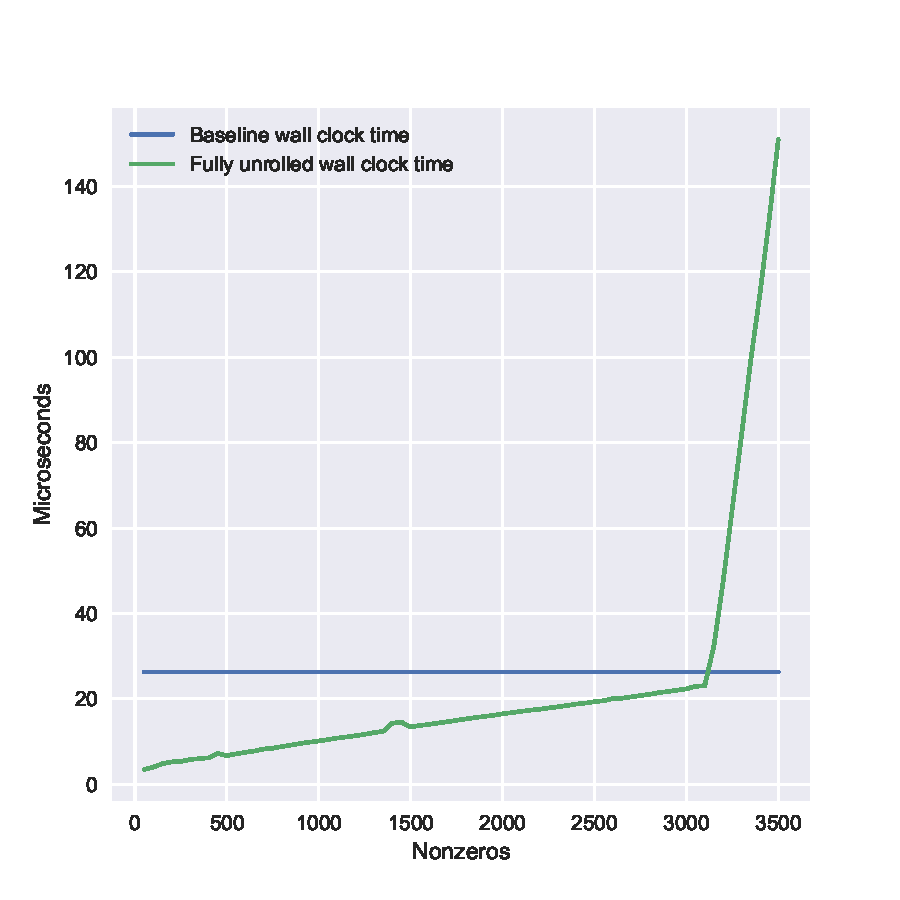
\includegraphics[width=5cm]{images/unrolled_scaling_time.pdf}
    \end{column}
    \begin{column}{0.45\textwidth}
      \centering
      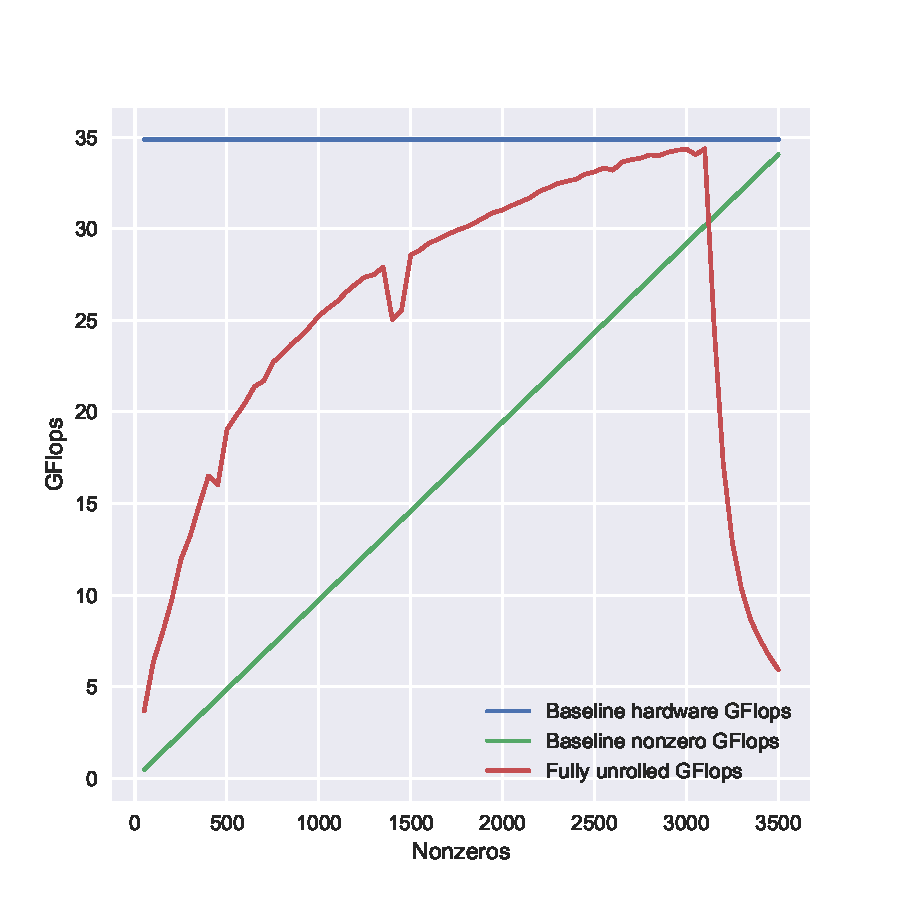
\includegraphics[width=5cm]{images/unrolled_scaling_flops.pdf}
    \end{column}
  \end{columns}

  \begin{itemize}
    \item For $nnz < 3100$, time-to-solution scales linearly.
    \item For $nnz > 3200$, the FMAs completely fill the instruction cache (regardless of matrix dimensions!)
    \item Fully unrolled sparse algorithm outperforms dense ``nonzero'' GFlops, but always underperforms dense ``hardware'' GFlops
    
  \end{itemize}
\end{frame}




\begin{frame}[fragile]
  \frametitle{Algorithm: General Sparse}
  Bypass the instruction cache limit by compressing the sparsity pattern. Decompose the matrix into blocks, fill in zeros to reduce the number of distinct block patterns, generate a microkernel for each \emph{distinct} block pattern. Traverse the block structure, jumping to the correct microkernel for each block. 


\def\r{\color{red}}
\def\g{\color{brown}}
\def\b{\color{blue}}


  \begin{columns}[t]
    \begin{column}{0.3\textwidth}
      \[\left[
          \begin{array}{ccc|ccc}
          \b* &   &   &    &    &    \\
            & \b* &   &    &    &    \\
          \b* &   & \b* &    &    &    \\
          \hline
          \r* &   &   & \g* &   & \g*  \\
          \r* & \r* &   &   & \g* &    \\
            & \r* & \r* &   &   & \g*  \\
          \end{array}
          \right]\]
        \footnotesize
        \begin{itemize}
          \item Distinct blocks = 3
          \item Jumps = 3
          \item Nonzeros = 13
          \item Density = 36\%
          \item FMAs = 13
        \end{itemize}
    \end{column}
    \begin{column}{0.3\textwidth}
      \[
      \left[
          \begin{array}{ccc|ccc}
          \b* &   & \b0 &    &    &    \\
            & \b* &   &    &    &    \\
          \b* &   & \b* &    &    &    \\
          \hline
          \r* &   &   & \b* &   & \b*  \\
          \r* & \r* &   &   & \b* &    \\
            & \r* & \r* & \b0 &   & \b*  \\
          \end{array}
          \right] \]

        \footnotesize
        \begin{itemize}
          \item Distinct blocks = 2
          \item Jumps = 3
          \item Nonzeros = 15
          \item Density = 42\%
          \item FMAs = 10
        \end{itemize}
    \end{column}
    \begin{column}{0.3\textwidth}
    \[
    \left[
          \begin{array}{ccc|ccc}
          \b* &   & \b0 &    &    &    \\
          \b0 & \b* &   &    &    &    \\
          \b* & \b0 & \b* &    &    &    \\
          \hline
          \b* &   & \b0 & \b* &   & \b*  \\
          \b* & \b* &   & \b0 & \b* &    \\
          \b0 & \b* & \b* & \b0 & \b0 & \b*  \\
          \end{array}
          \right]
      \]
          \footnotesize
          \begin{itemize}
          \item Distinct blocks = 1
          \item Jumps = 3
          \item Nonzeros = 21
          \item Density = 58\%
          \item FMAs = 7
        \end{itemize}
    \end{column}
  \end{columns}

\end{frame}

\begin{frame}[fragile]
  \frametitle{Algorithm: General Sparse}
  Implement this using a \emph{jump table} to efficiently dispatch to the correct microkernel. Unroll the block traversal into the instruction stream. This gives our matrix a sparse-outer, sparse-inner structure.


  \begin{columns}[t]%[onlytextwidth]
    \begin{column}{0.4\textwidth}
      \begin{itemize}
  \item[$+$] Takes advantage of shared structure in sparsity pattern
  \item[$+$] Minimizes fill-in

  \item[$-$] Time penalty for each jump: Limits total number of non-empty blocks.
  \item[$-$] Matrix must be stored in a format where blocks are continguous
  \item[$-$] Difficult to find best parameters automatically
      \end{itemize}
    \end{column}
    \begin{column}{0.6\textwidth}
      \begin{ccode}[]
        {text}
        unroll over each distinct pattern:

           declare unique gemm label
           blockwise C += A * B for that pattern
           indirect jump via return address register

        loop over m blocks:
           unroll over n blocks:

              load C block into registers
              unroll loop over k blocks:

                 if current B block is not empty:

                    move A, B to correct block
                    load return address label into register
                    direct jump to corresponding gemm label
                    declare label for return address

              store C block from registers
              move C right 1 block

           move A to next m panel
           move C down 1 block
      \end{ccode}
    \end{column}
  \end{columns}

\end{frame}


\begin{frame}[fragile]
  \frametitle{Results: Compressed Dense-by-Sparse Scaling}
  How do the number of jumps affect the performance of GeneralSparse?

  Choose matrix sizes $m=n=k=64$, block sizes $bm=bn=8, bk\in \{4,8,16\}.$ 
  B is randomly filled with $nnz\in\{400,800,...\}$. No compression was used.

  \centering
  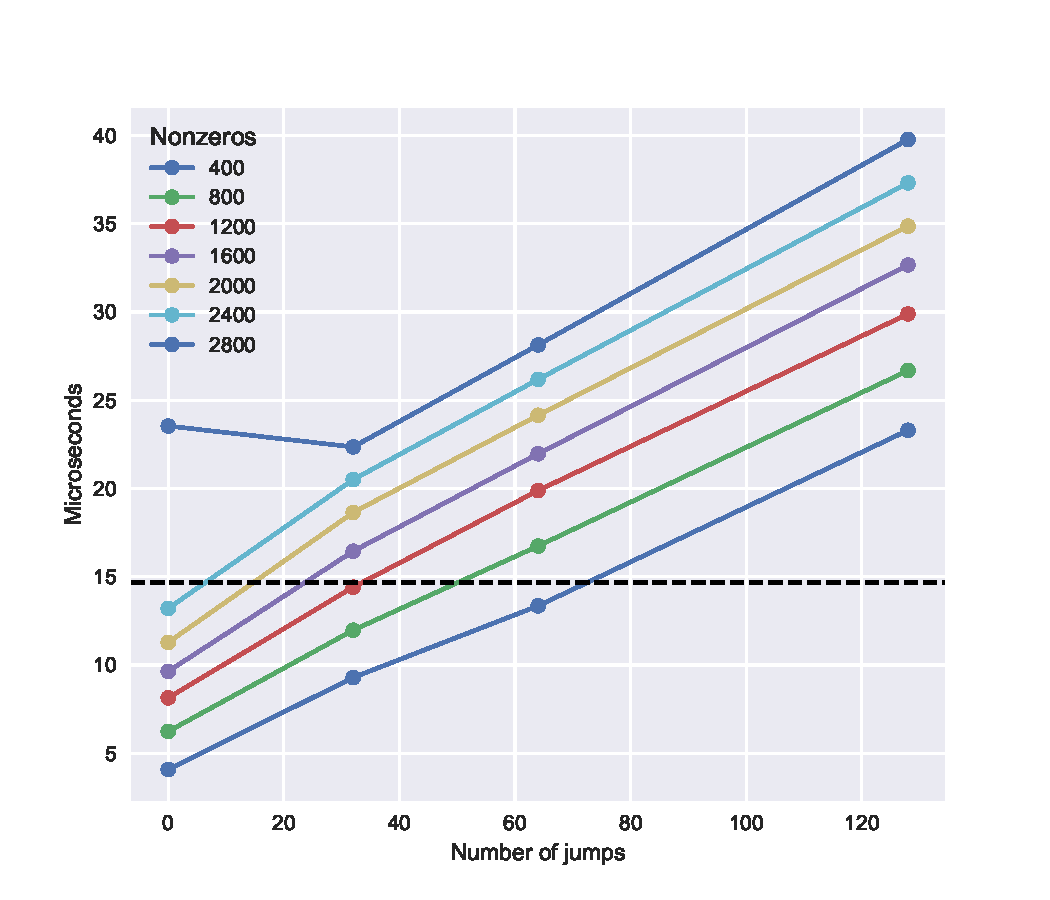
\includegraphics[height=5.5cm]{images/jump_penalty_new.pdf}

  \begin{itemize}
  \item Penalty is about 0.2 microseconds/jump
  \item Penalty does \emph{not} vary strongly with number of nonzeros
  \item Larger blocksizes needed for this to be effective $\implies$ Use UnrolledSparse as microkernel instead
  \end{itemize}

\end{frame}


\begin{frame}
  \frametitle{A family of dense-by-sparse algorithms}
  

\usetikzlibrary{shapes,arrows}
\usetikzlibrary{decorations.pathreplacing}


% Define block styles
\tikzstyle{decision} = [diamond, draw, fill=blue!20, 
    text width=4.5em, text badly centered, node distance=3cm, inner sep=0pt]

\tikzstyle{block} = [rectangle, draw, fill=gray!20, 
    text width=7em, text centered, minimum height=3em]

\tikzstyle{line} = [draw, -latex']

\tikzstyle{cloud} = [draw, ellipse,fill=red!20, node distance=3cm,
    minimum height=2em]

\begin{tikzpicture}[node distance = 5em, auto]
    % Place nodes

    \node [block] (microkernel) {Sparse\\ microkernel};
    \node [block, left of=microkernel, node distance=10em] (libxsmm) {Libxsmm dense outer product};
    \node [block, below of=microkernel] (macrokernel) {Unrolled sparse};
    \node [block, below of=macrokernel] (tiledsparse) {Tiled sparse};
    \node [block, right of=tiledsparse, node distance=10em] (blocksparse) {Block sparse};
    \node [block, below of=tiledsparse] (paddedsparse) {Padded sparse};
    \node [block, below of=blocksparse] (generalsparse) {General sparse};
    \node [block, below of=paddedsparse] (paddeddiagsparse) {Padded sparse with extracted diagonal};

    %\node [block, left of=evaluate, node distance=3cm] (update) {update model};
    %\node [decision, below of=evaluate] (decide) {is best candidate better?};
    %\node [block, below of=decide, node distance=3cm] (stop) {stop};

    % Draw edges
    \path [line] (libxsmm) -- (microkernel);
    \path [line] (microkernel) -- (macrokernel);
    \path [line] (macrokernel) -- (tiledsparse);
    \path [line] (tiledsparse) -- (blocksparse);
    \path [line] (tiledsparse) -- (paddedsparse);
    \path [line] (paddedsparse) -- (generalsparse);
    \path [line] (blocksparse) -- (generalsparse);
    \path [line] (paddedsparse) -- (paddeddiagsparse);

    \draw [decorate,decoration={brace,amplitude=10pt},xshift=0pt,yshift=0pt]
(1.75,-2) -- (4.75,-2)node [black,midway,yshift=9pt] {\footnotesize Irregular block offset};

    \draw [decorate,decoration={brace,amplitude=10pt},xshift=0pt,yshift=0pt]
(-2,-7.25) -- (-2,-4.25) node [black,midway,xshift=-8pt,text width=5em] {\footnotesize Multiple\\ Microkernels};
    %\path [line] (evaluate) -- (decide);
    %\path [line] (decide) -| node [near start] {yes} (update);
    %\path [line] (update) |- (identify);
    %\path [line] (decide) -- node {no}(stop);
    %\path [line,dashed] (expert) -- (init);
    %\path [line,dashed] (system) -- (init);
    %\path [line,dashed] (system) |- (evaluate);
\end{tikzpicture}



\end{frame}


\begin{frame}[fragile]
  \frametitle{Implementation}

  \begin{block}{Code Generation}
    \begin{itemize}
    \item Python domain-specific language for directly generating assembly
    \item Includes rich assembly AST: \texttt{Operand} $\leftarrow$ \texttt{Statement} $\leftarrow$ \texttt{Block} 
    \item Higher-level forms such as loops, subroutines, and jump tables
          implemented as plain Python functions which return a \texttt{Block}
    \item Pretty-printing, analysis, simulation are implemented using Visitor Pattern
    \item Interesting theoretical problem: Moving information from runtime to compile time in a general way
    \end{itemize}
  \end{block}



  \begin{block}{Matrix Cursor}
    A high-level abstraction for traversing and examining a sparse blocked matrix using \emph{logical coordinates}, automatically computing the physical memory offsets. Abstracts different sparsity patterns, block decompositions, sparse matrix formats, and memory addressing schemes.
    \begin{itemize}
    \item \verb|has_nonzero_block(pointer, block_coords) -> bool|
    \item \verb|has_nonzero_cell(pointer, cell_coords) -> bool|
    \item \verb|move(pointer, block_coords) -> (new_pointer, statement)|
    \item \verb|look(pointer, cell_coords) -> (new_pointer, memory_address)|
    \end{itemize}
    \end{block}
\end{frame}


\begin{frame}[fragile]
  \frametitle{Results: Speedup for various SeisSol matrices}

  

  \centering
  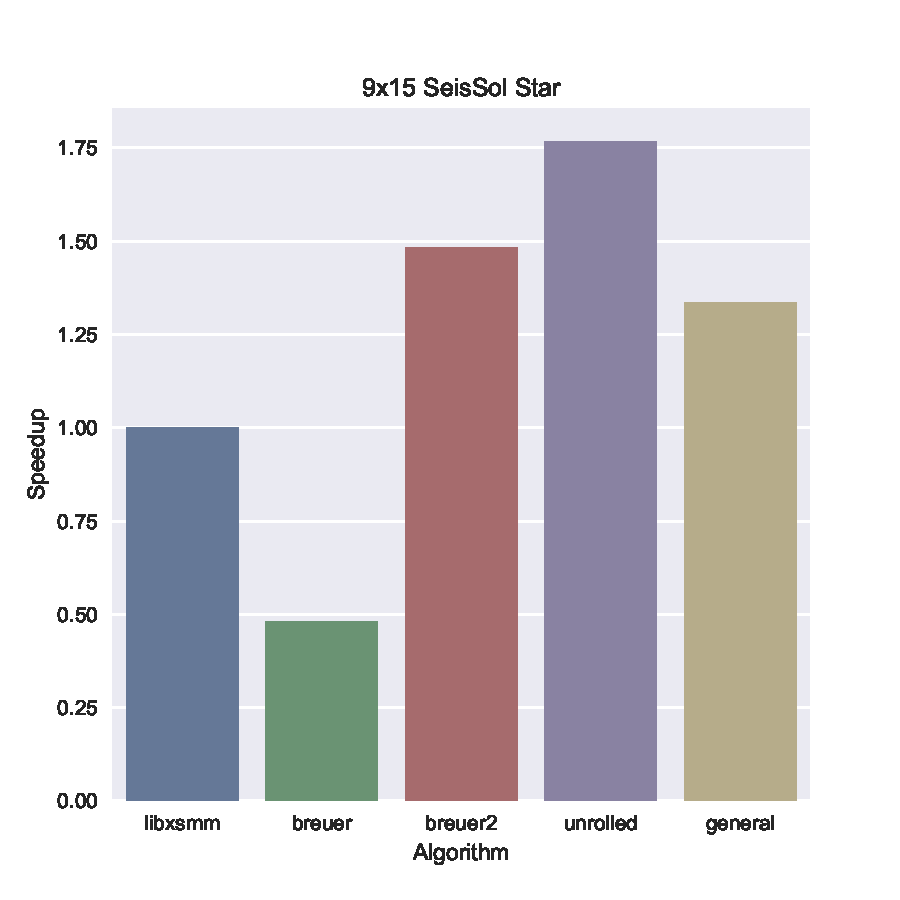
\includegraphics[height=6cm]{images/seissol_comparison.pdf}

  \begin{itemize}
  \item[$+$] We can reuse a single microkernel, reducing the number of instructions
  \item[$+$] The zero blocks reduce the number of filled-in nonzeros.
  \item[$-$] We can no longer visit blocks by using a loop with pointer arithmetic.
  \end{itemize}
\end{frame}



\begin{frame}[fragile]
  \frametitle{Outlook}

  \begin{block}{Tensor-by-sparse products}
  Idea: Fuse 8 simultaneous simulations, vectorizing along the third dimension.
    \begin{itemize}
    \item Sparse-by-dense is symmetric with dense-by-sparse
    \item Resulting algorithm resembles scalar matrix multiplication
    \item Already done in EDGE
    \end{itemize}
  \end{block}

  \begin{block}{Sparse-by-dense matrix products}
  This is significantly more difficult, but there are two approaches:
    \begin{enumerate}
    \item Keep outer-product formulation. Transpose the register blocks.
    \item Abandon outer-product formulation. One possible idea: Vectorize along sparse matrix diagonals; perform an inner-product and shift.
    \end{enumerate}
  \end{block}

  \begin{block}{Libxsmm proxy}
  Idea: Make these usable in a general way
    \begin{itemize}
    \item Handle different values of alpha, beta; prefetching. 
    \item Extend GeneralSparse to handle larger block sizes
    \item Algorithm for autochoosing the best GeneralSparse block sizes and fill-ins.
    \end{itemize}
  \end{block}

\end{frame}




\begin{frame}[plain,c]
\begin{center}
    \huge Thank you!
\end{center}
\end{frame}



\begin{frame}[fragile]
  \frametitle{Algorithm: Tiled Sparse}
        Assume there exists a sparse pattern which tiles perfectly over B.
        \begin{itemize}
        \item[$+$] We can reuse a single microkernel, reducing the number of instructions
        \item[$+$] We can visit blocks in a loop efficiently, using pointer tricks to reduce instruction size.
        \item[$-$] This regularity assumption is likely too strong.
        \item[$-$] In practice, the sparsity pattern would often become dense.
        \end{itemize}


      \[
      \left[
          \begin{array}{c c c | c c c }
          0 &   &   & 10 &   &   \\
          1 & 2 &   & 11& 12&   \\
            & 3 & 4 &   & 13& 14  \\
          \hline
          5 &   &   & 15  &   &   \\
          6 & 7 &   & 16  &17   &   \\
            & 8 & 9 &   & 18  &19   \\
          \end{array}
          \right]
      \]
\end{frame}

\begin{frame}[fragile]
  \frametitle{Algorithm: Block Sparse}
  Assume that B is decomposed into blocks which are either empty or `full'. `Full' blocks all have the same sparsity pattern. This is a sparse generalization of the block-sparse-column format.

  \begin{itemize}
  \item[$+$] We can reuse a single microkernel, reducing the number of instructions
  \item[$+$] The zero blocks reduce the number of filled-in nonzeros.
  \item[$-$] We can no longer visit blocks by using a loop with pointer arithmetic. \\Our options are:
    \begin{itemize}
    \item Look up the block location from a table in memory
    \item Unroll the block locations into the instruction stream and repeatedly jump to the microkernel.
    \end{itemize}
  \end{itemize}


      \[
      \left[
          \begin{array}{c c c | c c c }
          0 &   &   &    &    &    \\
          1 & 2 &   &    &    &    \\
            & 3 & 4 &    &    &    \\
          \hline
          5 &   &   & 10 &    &    \\
          6 & 7 &   & 11 & 12 &    \\
            & 8 & 9 &    & 13 & 14 \\
          \end{array}
          \right]
      \]
\end{frame}


\end{document}
